%%=============================================================================
%% Appendix Code AutoKeras
%%=============================================================================
\chapter{Code AutoKeras}
\label{ch:app:autokeras}

De code in deze bijlage werd gebruikt om beide AutoKeras modellen te trainen. Verder bevat het ook alle nodige informatie om feedback op te vragen van een getraind model en een manier om data te structureren en eenmalig in te laden. AutoKeras is nog volop in ontwikkeling waardoor deze code gevoelig is voor aanpassingen. Het gebruikt de aangeraden standaarden maar kan perfect op een andere manier geïmplementeerd worden. Die keuze hangt meestal af van de andere \textit{tools} die een ontwikkelaar gebruikt (Tensorflow dataset slices, \textit{multi task}...) en welke taak hij moet uitvoeren.

De versie van AutoKeras die tijdens dit onderzoek gebruikt werd bevatte een \textit{bug} die ongewenst gedrag \textit{triggerde} in \textit{greedy search} algoritmes wanneer het aantal pogingen groter was dan vijf. Er is een alternatieve versie voorzien dat \textit{random search} gebruikt. Beide methodes werden besproken in Hoofdstuk \ref{ch:autokeras}.

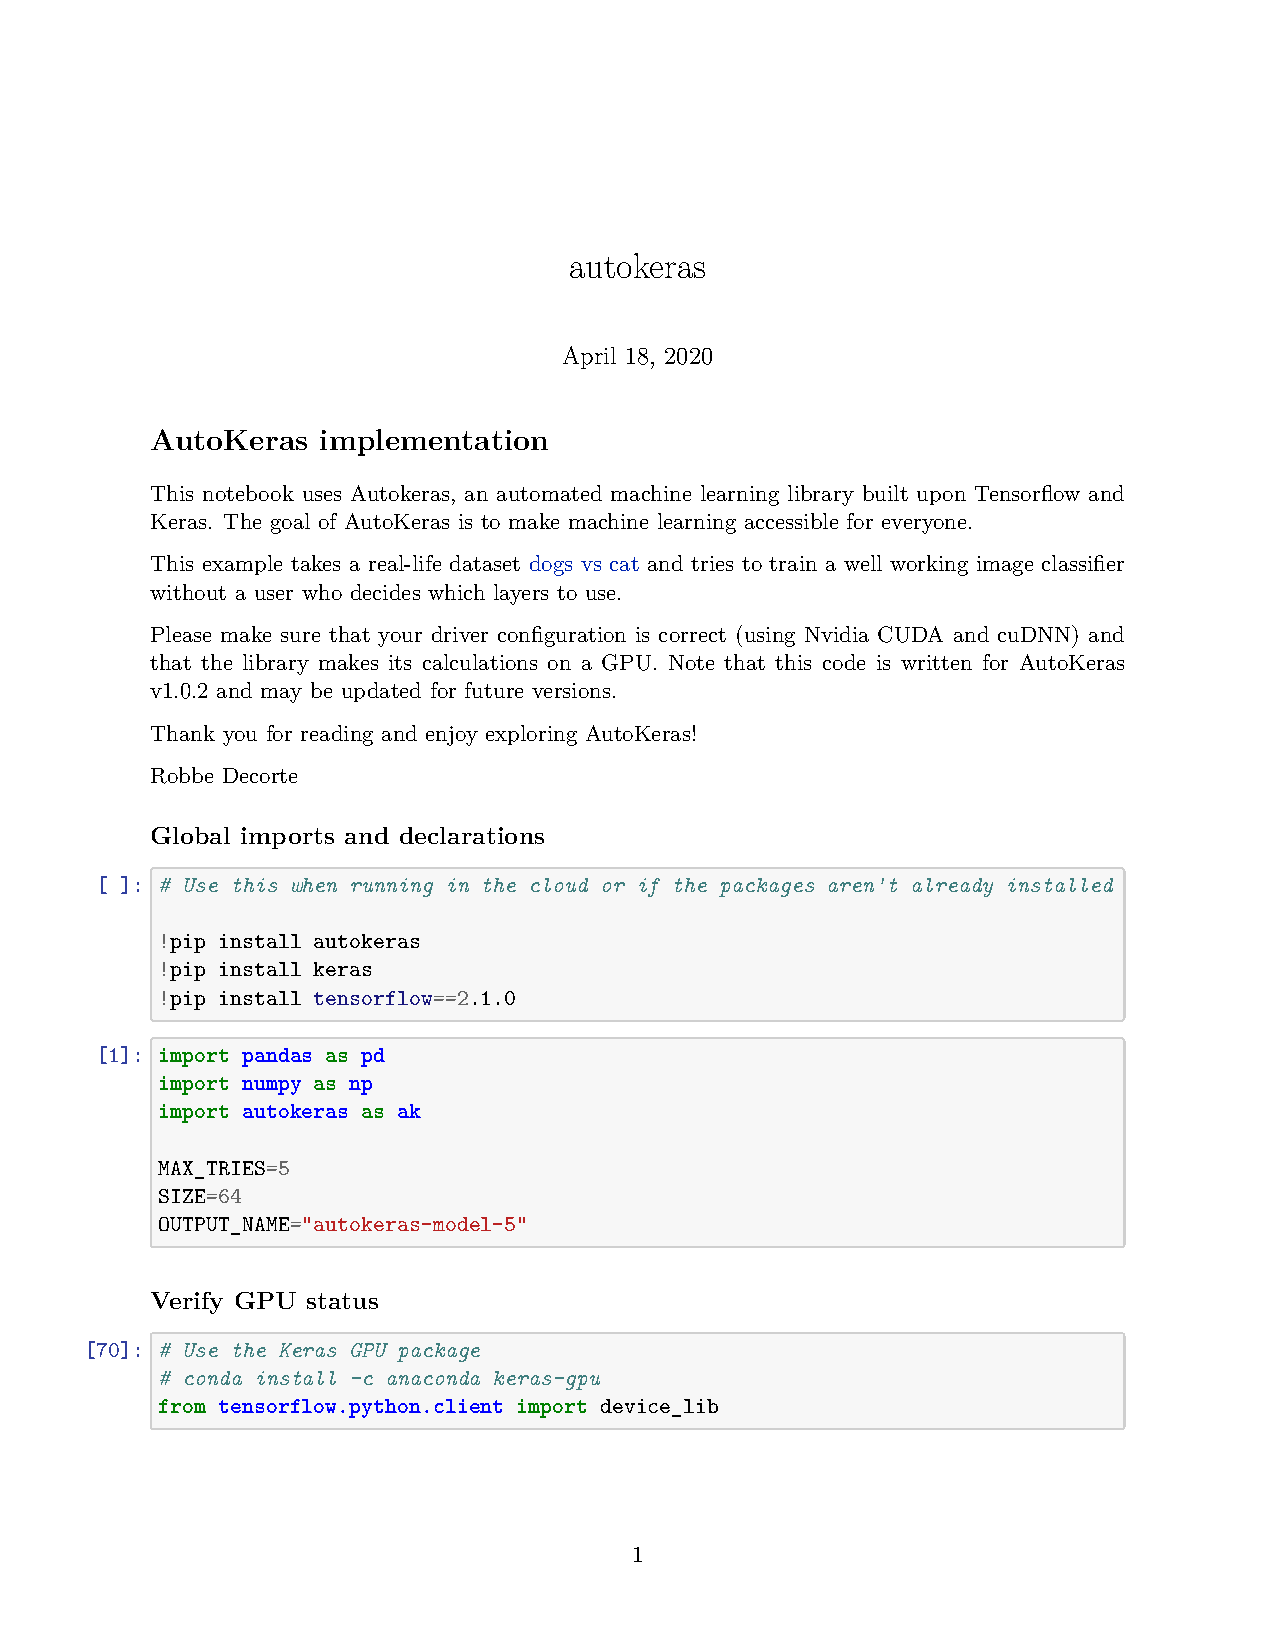
\includepdf[pages=-]{./nbconvert/autokeras.pdf}
